\subsection{Overall approach}
\label{sxn:approach}


Consider the objective/optimization function (parameterized by $\mathbf{W}_{l}$s and $\mathbf{b}_{l}$s) for a DNN with $L$ layers, activation functions $h_{l}(\cdot)$, and $N\times M$ weight matrices $\mathbf{W}_{l}$ and biases $\mathbf{b}_{l}$, as 
the minimization of a general Loss Function $\mathcal{L}$ over $N$ training data instances and labels, $\{\mathbf{x}_{i},y_{i}\}\in\mathcal{D}$.
For a typical supervised classification problem, one has
\begin{equation}
\underset{\mathbf{W}_{l},\mathbf{b}_{L}}{\text{argmin}}\;\sum_{i=1}^{N}\left(\mathcal{L}(E_{DNN}(\mathbf{x}_{i})-y_{i})\right)  ,
\end{equation}
where the loss function $\mathcal{L}(\cdot)$ can take on a myriad of forms~\cite{JC17_TR}, and where
\begin{equation}
E_{DNN}=h_{L}(\mathbf{W}_{L}\times h_{L-1}(\mathbf{W}_{L-1}\times h_{L-2}(\cdots)+\mathbf{b}_{L-1})+\mathbf{b}_{L})
\label{eqn:dnn_energy}
\end{equation}
is the Energy (or optimization) Landscape function.  
\michael{See comments for math equations, explain $h_{L}$, scalar valued function, $b_L$, times symbol, etc., confusing about role or $y$, and whether we are dealing with products of matrices.  E.g., $L$ layers, with activation functions $h_{l}(\cdot)$, and with $N\times M$ weight matrices $\mathbf{W}_{l}$ and biases $\mathbf{b}_{l}$; etc.  }
$E_{DNN}$ does not explicitly depend on the data, but rather it maps data instance vectors ($\mathbf{x}_i$ values) to predictions (labels).
\michael{Mark found that sentence confusing.}
Therefore, one can analyze $E_{DNN}$ in the absence of any training or test~data. 

Test accuracies have been reported online for publicly-available pretrained pyTorch models~\cite{osmr}.
These models have been trained and evaluated on labeled data $\{\mathbf{x}_{i},y_{i}\}\in\mathcal{D}$, using standard techniques.  
We do not have access to this data, and we have not trained any of the models ourselves. 
Our methodological approach is thus similar to a statistical meta-analysis, common in biomedical research, but uncommon in ML.
%
Computations were performed with the publicly-available \texttt{WeightWatcher} tool (version 0.2.7)~\cite{weightwatcher_package}.
To be fully reproducible, we only examine publicly-available, pretrained models, and we provide all Jupyter and Google Colab notebooks used in an accompanying github repository~\cite{kdd20_sub_repo}.
See the Supplementary Information
%~\ref{sxn:appendix} 
for details.


\paragraph{Metrics for DNN Weight Matrices.}

Our approach involves analyzing individual DNN weight matrices, for (depending on the architecture) fully-connected and/or convolutional layers.
Each DNN layer contains one or more layer 2D  $N\times M$ weight matrices, $\mathbf{W}_{l}$, or pre-activation maps, $\mathbf{W}_{i,l}$, e.g., extracted from 2D Convolutional layers, where $N > M$.
See the Supplementary Information
%~\ref{sxn:appendix} 
for details.
(We may drop the $i$ and/or $i,l$ subscripts below.)
The best performing quality metrics depend on the norms and/or spectral properties of each weight matrix,
$\mathbf{W}$, and/or, equivalently, it's Empirical Correlation Matrix, $\mathbf{X}=\mathbf{W}^{T}\mathbf{W}$.
We consider the following metrics:
\begin{eqnarray}
& & \text{Frobenius Norm: $\Vert\mathbf{W}\Vert^{2}_{F}=\Vert\mathbf{X}\Vert_{F}=\sum\nolimits_{i=1}^{M} \lambda_{i}$ } \\
& & \text{Spectral Norm: $\Vert\mathbf{W}\Vert_{\infty}^{2}=\Vert\mathbf{X}\Vert_{\infty}=\lambda_{max}$ } \\
& & \text{Weighted Alpha: $\hat{\alpha}=\alpha\log\lambda_{max}$ } \\
& & \text{$\alpha$-Norm (or $\alpha$-Shatten Norm): $\Vert\mathbf{W}\Vert^{2\alpha}_{2\alpha}=\Vert\mathbf{X}\Vert^{\alpha}_{\alpha}=\sum\nolimits_{i=1}^{M}\lambda_{i}^{\alpha}$. }
\end{eqnarray}
Here, $\lambda_{i}$ is the $i^{th}$ eigenvalue of the $\mathbf{X}$, and $\lambda_{max}$ is the maximum eigenvalue.
These eigenvalues are squares of the singular values $\sigma_{i}$ of $\mathbf{W}$, $\lambda_{i}=\sigma^{2}_{i}$.
All four metrics can be computed easily from DNN weight matrices.
The first two metrics are well-known in ML.
The last two metrics deserve special mention, as they depend on an empirical parameter $\alpha$ that is the PL exponent that arises in the recently-developed Heavy Tailed Self Regularization (HT-SR) Theory~\cite{MM18_TR, MM19_HTSR_ICML, MM20_SDM}.


\paragraph{Overview of Heavy-Tailed Self-Regularization.}

In the HT-SR Theory, one analyzes the eigenvalue spectrum, i.e., the Empirical Spectral Density (ESD), of the associated correlation matrices~\cite{MM18_TR,MM19_HTSR_ICML,MM20_SDM}.
From this, one characterizes the amount and form of correlation, and therefore implicit self-regularizartion, present in the DNN's weight matrices.
For each layer weight matrix $\mathbf{W}$, of size $N \times M$, construct the associated $M\times M$ (uncentered) correlation matrix $\mathbf{X}$. 
Dropping the $L$ and $l,i$ indices, one~has
$$
\mathbf{X} = \frac{1}{N}\mathbf{W}^{T}\mathbf{W}.
$$
If we compute the eigenvalue spectrum of $\mathbf{X}$, i.e., $\lambda_i$ such that
$  % $$
\mathbf{X}\mathbf{v}_{i}=\lambda_{i}\mathbf{v}_{i} , 
$  % $$
then the ESD of eigenvalues, $\rho(\lambda)$, is just a histogram of the eigenvalues, formally written as
%\begin{equation}
$\rho(\lambda)=\sum\nolimits_{i=1}^{M}\delta(\lambda-\lambda_{i})  .$
%\label{eqn:eigenval_hist}
%\end{equation}
Using HT-SR Theory, one characterizes the correlations in a weight matrix by examining its ESD, $\rho(\lambda)$.
It can be well-fit to a truncated PL distribution, given~as
\begin{equation}
\rho(\lambda)\sim\lambda^{-\alpha}  ,
\label{eqn:eigenval_pl}
\end{equation}
which is (at least) valid within a bounded range of eigenvalues $\lambda\in[\lambda^{min},\lambda^{max}]$.  

The original work on HT-SR Theory considered a small number of NNs, including AlexNet and InceptionV3. 
It showed that for nearly every $\mathbf{W}$, the (bulk and tail) of the ESDs can be fit to a truncated PL, and that PL exponents $\alpha$ nearly all lie within the range $\alpha\in(1.5,5)$~\cite{MM18_TR,MM19_HTSR_ICML,MM20_SDM}.
%
As for the mechanism responsible for these properties, statistical physics offers several possibilities~\cite{SornetteBook,nishimori01}, e.g., self organized criticality~\cite{SOC87,SOCat25yrs} or multiplicative noise in the stochastic optimization algorithms used to train these models~\cite{HodMah20A_TR,SorCon97}.
Our meta-analysis does not require knowledge of mechanisms; and it is not even clear that one mechanism is responsible for every case.
%
Crucially, HT-SR Theory predicts that smaller values of $\alpha$ should correspond to models with better correlation over multiple size scales and thus to better models.
Relatedly, previous work observed that smaller exponents $\alpha$ correspond to more implicit self-regularization and better generalization~\cite{MM18_TR,MM19_HTSR_ICML,MM20_SDM}.


\paragraph{DNN Empirical Quality Metrics.}

For norm-based metrics, we use the average of the log norm, to the appropriate power.
Informally, this amounts to assuming that the layer weight matrices are statistically independent, in which case we can estimate the model complexity $\mathcal{C}$, or test accuracy, with a standard Product Norm (which resembles a data dependent VC complexity),
\begin{equation}
\mathcal{C}\sim\Vert\mathbf{W}_{1}\Vert\times\Vert\mathbf{W}_{2}\Vert \times \cdots \times \Vert\mathbf{W}_{L}\Vert ,
\end{equation}
where $\Vert\cdot\Vert$ is a matrix norm.   
The log complexity,
\begin{equation}
\label{eqn:eqn:sum_log_norm}
\log\mathcal{C} \sim \log\Vert\mathbf{W}_{1}\Vert+\log\Vert\mathbf{W}_{2}\Vert + \cdots + \log\Vert\mathbf{W}_{L}\Vert = \sum\nolimits_l \log\Vert\mathbf{W}_{l}\Vert ,
\end{equation}
 takes the form of an average Log Norm.
For the Frobenius Norm metric and Spectral Norm metric, we can use Eqn.~(\ref{eqn:eqn:sum_log_norm}) directly (since, when taking $\log\Vert\mathbf{W}_{l}\Vert_{F}^{2}$, the $2$ comes down and out of the sum, and thus ignoring it only changes the metric by a constant factor).


The Weighted Alpha metric is an average of $\alpha_l$ over all layers $l \in \{1,\ldots,l\}$, weighted by the size, or scale, or each matrix,
\begin{equation}
\hat{\alpha} = \dfrac{1}{L}\sum_l \alpha_l\log\lambda_{max,l}\approx\langle\log\Vert\mathbf{X}\Vert_{\alpha}^{\alpha}\rangle    ,
\end{equation}
where $L$ is the total number of layer weight matrices.
The Weighted Alpha metric was introduced previously~\cite{MM20_SDM}, where it was shown to correlate well with trends in reported test accuracies of pretrained DNNs, albeit on a much smaller and more limited set of models than we consider here.

Based on this, in this paper, we introduce and evaluate the $\alpha$-Shatten Norm metric,
\begin{equation}
\label{eqn:sum_log_alpha_norm_alpha}
\sum\nolimits_l \log \Vert\mathbf{X}_l\Vert_{\alpha_l}^{\alpha_l} 
=
\sum\nolimits_l \alpha_l \log \Vert\mathbf{X}_l\Vert_{\alpha_l} .
\end{equation}
For the $\alpha$-Shatten Norm metric, $\alpha_l$ varies from layer to layer, and so in Eqn.~(\ref{eqn:sum_log_alpha_norm_alpha}) it can not be taken out of the sum.
For small $\alpha$, the Weighted Alpha metric approximates the Log $\alpha$-Shatten norm, as can be shown with a statistical mechanics and random matrix theory derivation \cite{MM20_unpub_work}; and the Weighted Alpha and $\alpha$-Shatten norm metrics often behave like an improved, weighted average Log Spectral Norm.


One determines $\alpha$ for a given layer by fitting the ESD of that layer's weight matrix to a truncated PL, using the commonly accepted Maximum Likelihood method~\cite{CSN09_powerlaw,ABP14}.
This method works very well for exponents between $\alpha\in(2,4)$; and it is adequate, although imprecise, for smaller and especially larger $\alpha$~\cite{newman2005_zipf}. 
%
Operationally, $\alpha$ is determined by using the \texttt{WeightWatcher} tool~\cite{weightwatcher_package} to fit the histogram of eigenvalues, $\rho(\lambda)$, to a truncated PL, 
\begin{equation}
\rho(\lambda)\sim\lambda^{\alpha},\;\;\lambda\in[\lambda_{min},\lambda_{max}] ,
\end{equation}
where $\lambda_{max}$ is the largest eigenvalue of $\mathbf{X}=\mathbf{W}^{T}\mathbf{W}$, and 
where $\lambda_{min}$ is selected automatically to yield the best (in the sense of minimizing the K-S distance) PL fit.
Each of these quantities is defined for a given layer $\mathbf{W}$ matrix.
See Figure~\ref{fig:ww} for an illustration.

\begin{figure}[t]
    \centering
    \includegraphics[width=15.0cm]{img/WeightWatcher_v2}
    %\includegraphics[width=15.0cm]{../img2/WeightWatcher_v2}
    \caption{Schematic of analyzing DNN layer weight matrices $\mathbf{W}$.  
             Given an individual layer weight matrix $\mathbf{W}$, from either a fully-connected layer or a convolutional layer, perform a Singular Value Decomposition (SVD) to obtain $\mathbf{W} = \mathbf{U} \mathbf{\Sigma} \mathbf{V}^{T}$, and examine the histogram of eigenvalues of $\mathbf{W}^{T}\mathbf{W}$.
             Norm-based metrics (not shown) and PL-based metrics (that depend on fitting the histogram of eigenvalues to a truncated PL) can be used to compare models.
             For example, one can analyze one layer of a pre-trained model, compare multiple layers of a pre-trained model, make comparisons across model architectures, monitor neural network properties during training, etc. 
             \michael{Put the Analyze, Compare, Monitor comments in the caption, not the figure.}
}
    \label{fig:ww}
\end{figure}



To avoid confusion, let us clarify the relationship between $\alpha$ and $\hat{\alpha}$.  
We fit the ESD of the correlation matrix $\mathbf{X}$ to a truncated PL, parameterized by 2 values: the PL exponent $\alpha$, and the maximum eigenvalue $\lambda_{max}$.
The PL exponent $\alpha$ measures the amount of correlation in a DNN layer weight matrix $\mathbf{W}$. 
It is valid for $\lambda\le\lambda_{max}$, and it is scale-invariant, i.e., it does not depend on the normalization of $\mathbf{W}$ or $\mathbf{X}$.
The $\lambda_{max}$ is a measure of the size, or scale, of $\mathbf{W}$.
Multiplying each $\alpha$ by the corresponding $\log\lambda_{max}$ weighs ``bigger'' layers more, and averaging this product leads to a balanced, Weighted Alpha metric $\hat{\alpha}$ for the entire~DNN.


